\chapter{Pipeline de CI/CD}

\section{Ferramenta de versionamento}

\begin{table}[ht]
	\centering
	\resizebox{\textwidth}{!}{%
		\begin{tabular}{|c|c|c|c|}
			\hline
			\multirow{2}{*}{\textbf{Plataforma}} & \multicolumn{3}{c|}{\textbf{Comparação}}                                                                          \\ \cline{2-4}
			                                     & \textbf{GitHub}                          & \textbf{GitLab}             & \textbf{Bitbucket}                       \\ \hline

			\multirow{2}{*}{\textbf{Benefícios}}
			                                     & Comunidade ampla,                        & CI/CD integrado,            & Integração Atlassian,                    \\
			                                     & Marketplace extenso.                     & Privacidade gratuita.       & Repositórios privados gratuitos.         \\ \hline

			\multirow{2}{*}{\textbf{Desvantagens}}
			                                     & Preço por repositório privado,           & Interface menos intuitiva,  & Limitações em repositórios gratuitos,    \\
			                                     & Limitações de armazenamento.             & Recursos de hardware.       & Menos recursos de CI/CD.                 \\ \hline

			\multirow{2}{*}{\textbf{Uso Comum}}
			                                     & Projetos open-source,                    & Solução completa de DevOps, & Equipes usando Atlassian.                \\
			                                     & Colaboração em larga escala.             & Controle total sobre CI/CD. & Integração de gerenciamento de projetos. \\ \hline
		\end{tabular}%
	}
	\caption{Comparação entre GitHub, GitLab e Bitbucket}
	\label{tab:platform_comparison}
\end{table}

\par Será utilizado o GitHub para controle de versões e colaboração eficiente no desenvolvimento de software. Ele fornece um ambiente centralizado para armazenar, acompanhar e gerenciar código-fonte, facilita a colaboração de equipes distribuídas e ajuda a controlar mudanças e atualizações no código, tornando o processo de desenvolvimento mais organizado, transparente e eficaz.

\section{Servidor de CI/CD}
\begin{table}[ht]
	\centering
	\resizebox{\textwidth}{!}{%
		\begin{tabular}{|c|c|c|c|c|}
			\hline
			\multirow{2}{*}{\textbf{Critério}} & \multicolumn{4}{c|}{\textbf{Servidor de CI/CD}}                                                                                     \\ \cline{2-5}
			                                   & \textbf{Jenkins}                                & \textbf{TravisCI}         & \textbf{CircleCI}      & \textbf{AWS CodePipeline}    \\ \hline

			\textbf{Quando Usar}               & Projetos grandes com                            & Projetos open-source      & Projetos pequenos      & Projetos na AWS              \\
			                                   & necessidade de customização.                    & com diferentes ambientes. & com integração rápida. & com serviços AWS integrados. \\ \hline

			\textbf{Benefícios}                & Alta customização,                              & Integração rápida,        & Integração rápida,     & Integração com               \\
			                                   & pipelines codificáveis.                         & fácil configuração.       & fácil configuração.    & serviços AWS.                \\ \hline

			\textbf{Desvantagens}              & Complexo e demorado                             & Ideal para projetos       & Pode ser limitado para & Menos flexível com           \\
			                                   & para configurar.                                & menores.                  & projetos grandes.      & integrações de terceiros.    \\ \hline
		\end{tabular}%
	}
	\caption{Comparação entre Servidores de CI/CD}
	\label{tab:ci_cd_comparison}
\end{table}

A escolha do Jenkins como nossa ferramenta de CI/CD é estratégica devido à sua natureza de código aberto e à familiaridade preexistente da nossa equipe com ela. O caráter open source do Jenkins alinha-se com nosso valor de promover a transparência e flexibilidade, enquanto a familiaridade da equipe acelera a integração e minimiza a curva de aprendizado. Com uma comunidade ativa e um ecossistema robusto, o Jenkins oferece um ambiente confiável para automatizar nossos processos de desenvolvimento, tornando-se uma escolha sólida para nosso projeto.

\section{Tecnologias utilizadas}

Neste projeto, empregamos uma combinação de linguagens de programação, frameworks, bibliotecas e sistemas de gerenciamento de banco de dados para construir e gerenciar o sistema em diferentes camadas. A seguir, descrevemos as tecnologias utilizadas em cada camada:

\subsection{Front-end}
\begin{itemize}
	\item \textbf{Linguagem}: JavaScript - Uma linguagem de programação amplamente adotada para desenvolvimento web.
	\item \textbf{Framework}: React.js - Um popular framework JavaScript para construir interfaces de usuário interativas.
	\item \textbf{Estilo}: Bootstrap - Um framework CSS para desenvolver sites responsivos e projetos web móveis de primeira classe.
\end{itemize}

\subsection{Back-end Principal}
\begin{itemize}
	\item \textbf{Linguagem}: Python - Conhecida por sua legibilidade e eficiência.
	\item \textbf{Framework}: Flask - Um microframework web para Python.
	\item \textbf{Autenticação}: Flask-JWT-Extended - Uma extensão do Flask para lidar com a autenticação JWT (JSON Web Token).
\end{itemize}

\subsection{Microserviço de Processamento de Faturas}
\begin{itemize}
	\item \textbf{Linguagem}: Python.
	\item \textbf{Biblioteca de Análise de Dados}: Pandas - Usada para manipulação e análise eficiente dos dados das faturas.
	\item \textbf{Mensageria}: RabbitMQ - Facilita a comunicação assíncrona entre o microserviço e o back-end monolítico.
\end{itemize}


\subsection{Banco de Dados}
\begin{itemize}
	\item \textbf{SGBD}: PostgreSQL - Um sistema de gerenciamento de banco de dados relacional poderoso e de código aberto.
\end{itemize}

\section{Ferramentas de Build}
A seleção de uma ferramenta adequada para gerenciamento de dependências e construção do projeto é crucial para a eficiência do processo de desenvolvimento. Maven, Gradle e Docker são três tecnologias populares, cada uma com suas peculiaridades. Maven é conhecido por sua simplicidade e reprodutibilidade, Gradle por sua flexibilidade e desempenho, enquanto Docker destaca-se na criação e distribuição de contêineres. A tabela abaixo apresenta uma comparação entre essas tecnologias, visando auxiliar na escolha consciente da ferramenta mais alinhada às necessidades do projeto.

\begin{table}[ht]
	\centering
	\resizebox{\textwidth}{!}{%
		\begin{tabular}{|c|c|c|c|}
			\hline
			\multirow{2}{*}{\textbf{Critério}} & \multicolumn{3}{c|}{\textbf{Tecnologia}}                                                                       \\ \cline{2-4}
			                                   & \textbf{Maven}                           & \textbf{Gradle}         & \textbf{Docker}                           \\ \hline

			\textbf{Quando Usar}               & Projetos com                             & Projetos que necessitam & Quando a criação e                        \\
			                                   & estruturação clara.                      & de flexibilidade.       & distribuição de contêineres é necessária. \\ \hline

			\textbf{Benefícios}                & Simplicidade,                            & Flexibilidade,          & Portabilidade,                            \\
			                                   & reprodutibilidade.                       & desempenho.             & isolamento.                               \\ \hline

			\textbf{Desvantagens}              & Menos flexível,                          & Curva de aprendizado    & Requer conhecimento                       \\
			                                   & pode ser lento.                          & inicial.                & em contêineres.                           \\ \hline
		\end{tabular}%
	}
	\caption{Comparação entre Maven, Gradle e Docker}
	\label{tab:technology_comparison}
\end{table}

\par Contudo, optamos em utilizar o Docker como ferramenta de build, por oferecer vantagens como a criação de ambientes de construção consistentes, isolados e portáteis. Isso garante a reprodutibilidade, a segurança e a facilidade de integração com CI/CD. A decisão de usar o Docker depende do contexto e dos requisitos do projeto.

\section{Definição de Ferramentas e Estrutura de Execução para Deploy}

A implantação eficaz do \textit{Fintrackr} é crucial para garantir uma experiência de usuário contínua e robusta. Para alcançar essa eficiência, adotamos um conjunto de ferramentas líderes de mercado e definimos uma estrutura de execução que prioriza a escalabilidade, consistência e facilidade de manutenção.

\section{Ferramentas para Deploy}

A correta implantação do \textit{FinTrackr} é vital para garantir uma experiência de usuário suave e robusta. Para este fim, optamos por um conjunto de ferramentas líderes de mercado e estabelecemos uma estrutura de execução que prioriza a escalabilidade, consistência e facilidade de manutenção.

\begin{itemize}
	\item \textbf{GitHub}: Nossa escolha para controle de versões, o GitHub, permite uma colaboração eficaz e mantém um registro detalhado de todas as alterações no código, tornando o rastreamento e a reversão, quando necessário, um processo simplificado.
	\item \textbf{Jenkins}: Para a integração contínua e entrega contínua (CI/CD), optamos pelo Jenkins devido à sua flexibilidade, ampla comunidade de suporte e capacidade de integração com uma variedade de outras ferramentas, incluindo o Ansible e o Kubernetes.
\end{itemize}

\section{Estrutura de Execução}

A natureza modular e escalável do \textit{FinTrackr} se alinha perfeitamente com as capacidades fornecidas pelo Docker, uma plataforma de contêineres que permite empacotar, distribuir e executar aplicações de forma consistente e isolada. A utilização do Docker não apenas facilita o processo de desenvolvimento, mas também otimiza a operação e a distribuição da aplicação.

\subsection{Contêinerização e Isolamento}

O Docker proporciona um ambiente controlado e consistente para executar o \textit{FinTrackr}, isolando suas dependências e serviços associados em contêineres. Essa contêinerização assegura que o aplicativo se comportará da mesma maneira, independentemente de onde seja implantado, mitigando assim os problemas comuns de "funciona na minha máquina". Além disso, a isolamento fornecido pelos contêineres do Docker protege o \textit{FinTrackr} de possíveis interferências de outras aplicações ou serviços no mesmo ambiente.

\subsection{Desenvolvimento e Testes}

Durante as fases de desenvolvimento e testes, os desenvolvedores podem tirar proveito da facilidade de inicialização e descarte de contêineres Docker. Isso permite que eles configurem, testem e reconfigurem o ambiente do \textit{FinTrackr} de maneira rápida e sem esforço, acelerando o ciclo de desenvolvimento e garantindo que os testes sejam executados em um ambiente controlado e previsível.

\subsection{Integração e Entrega Contínua}

A integração do Docker com ferramentas de Integração Contínua/Entrega Contínua (CI/CD) adotado, o Jenkins, facilita a automação do pipeline de desenvolvimento do \textit{FinTrackr}. Os contêineres Docker podem ser construídos, testados e implantados automaticamente através de pipelines CI/CD, garantindo que cada alteração no código seja verificada e entregue de maneira eficaz e eficiente.

\subsection{Execução}

Para executar o \textit{FinTrackr} utilizando Docker, seguiremos uma estrutura padronizada:

\begin{enumerate}
	\item \textbf{Instalação do Docker}: O Docker será instalado no ambiente de execução desejado, seja um servidor local, um ambiente de nuvem ou uma máquina de desenvolvimento.
	\item \textbf{Criação de Imagens}: Imagens Docker serão criadas para cada componente do \textit{FinTrackr}, incluindo o back-end, front-end e o microserviço de processamento de faturas. Cada imagem será construída usando um Dockerfile que define as dependências, variáveis de ambiente e comandos necessários para executar o componente.
	\item \textbf{Construção de Imagens}: Usaremos o comando \textit{docker build} para construir as imagens a partir dos Dockerfiles.
	\item \textbf{Execução de Contêineres}: Os contêineres serão iniciados usando o comando \textit{docker run}, configurando as redes, volumes e outras opções necessárias para conectar os contêineres entre si e com os recursos externos necessários.
\end{enumerate}

\section{GitFlow}
O \textit{GitFlow} é uma estratégia de fluxo de trabalho do Git que define uma estrutura robusta para projetos, facilitando o desenvolvimento paralelo, a colaboração em equipe e o lançamento de versões estáveis. A estratégia é composta por várias \textit{branches} que têm propósitos específicos. A seguir, detalhamos essas \textit{branches} e suas interações:

\begin{itemize}
	\item \textbf{main}: Contém o código considerado como produção. Cada \textit{commit} nesta branch é uma nova versão de produção.

	\item \textbf{develop}: Atua como uma branch de integração para novos recursos e é o principal local de desenvolvimento contínuo.

	\item \textbf{feature branches}: Criadas a partir da branch \textit{develop}. São utilizadas para desenvolver novas funcionalidades sem afetar o código principal. Quando uma funcionalidade é concluída, um \textit{Pull Request} (PR) é criado para mesclar a \textit{feature branch} de volta à branch \textit{develop}.

	\item \textbf{hotfix branches}: Surgem a partir da branch \textit{main}. Destinadas para correções rápidas diretamente no código de produção. Quando uma correção é finalizada, PRs são abertos para integrar a \textit{hotfix branch} tanto na branch \textit{main} quanto na \textit{develop}.
\end{itemize}

Os \textit{Pull Requests} (PRs) desempenham um papel fundamental no GitFlow. Eles oferecem um ponto de revisão e teste, garantindo que o código seja de alta qualidade antes da integração. Esse processo de revisão é vital para a colaboração em equipe, permitindo que os membros da equipe revisem, comentem e testem as alterações propostas antes de serem incorporadas ao código base.

O GitFlow, com sua estrutura clara e regras definidas, ajuda as equipes a gerenciar e versionar seu código de forma eficaz, garantindo lançamentos estáveis e facilitando o desenvolvimento contínuo e a colaboração.

\begin{figure}[ht]
	\centering
	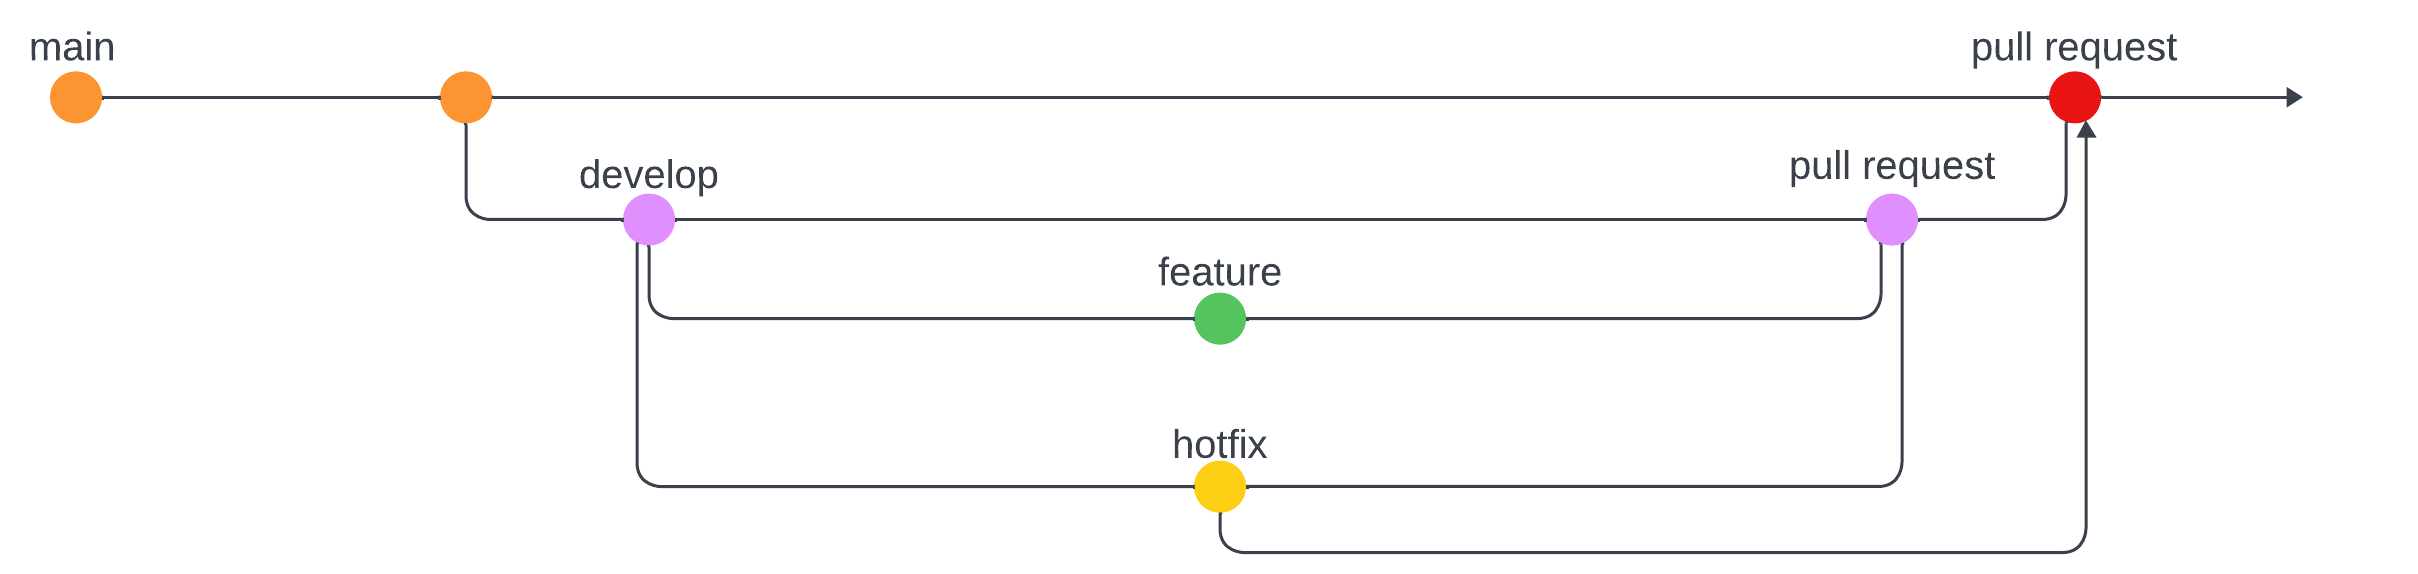
\includegraphics[width=1\linewidth]{Textuais/images/gitflow.png}
	\caption{\textit{GitFlow}}
	\label{fig:enter-label}
\end{figure}

\section{Testes}

\subsection{Ferramentas de Testes}
Para a linguagem Python será utilizado o Pytest, conhecido por sua sintaxe simples, identificação automática de testes, uso de fixtures, suporte a parametrização, extensibilidade por meio de plugins, e facilidade de integração com outras ferramentas de desenvolvimento. É amplamente adotado em projetos de código aberto e empresas, tornando o processo de teste eficiente e agradável para os desenvolvedores.

Para o React, será utilizado o Jest, ele é um framework de teste desenvolvido pelo Facebook que é amplamente usado na comunidade React. Ele é projetado para testar JavaScript, incluindo código React. O Jest é conhecido por sua simplicidade e integração perfeita com o React. Ele suporta testes de componentes, testes de unidades e testes de integração.

\subsection{Metrica de Cobertura de Testes}
A meta do nosso projeto é atingir uma cobertura de testes de 60\%. A cobertura de testes é fundamental para garantir a qualidade e a confiabilidade do nosso software. Com uma cobertura adequada, podemos identificar e corrigir erros de maneira eficaz, melhorar a manutenção do código e aumentar a confiança na estabilidade do sistema.

Para alcançar essa meta, planejamos implementar uma estratégia abrangente de testes que serão executados regularmente em um ambiente de integração contínua para garantir que nossa cobertura de testes seja mantida ao longo do tempo.

Atingir 60\% de cobertura de testes é um processo contínuo, e planejamos monitorar nosso progresso ao longo do ciclo de vida do projeto. Estabelecemos marcos específicos para avaliar nosso avanço e faremos ajustes conforme necessário para atender a essa meta.

Acreditamos que essa abordagem nos permitirá entregar um software de alta qualidade, com menos bugs e maior confiabilidade, beneficiando nossos usuários finais e nossa equipe de desenvolvimento.


\section{Artifacts Management}

\begin{table}[ht]
	\centering
	\resizebox{\textwidth}{!}{%
		\begin{tabular}{|c|c|c|c|c|}
			\hline
			\multirow{2}{*}{\textbf{Tecnologia}} & \multicolumn{4}{c|}{\textbf{Aspectos}}                                                                       \\ \cline{2-5}
			                                     & \textbf{Benefícios}                    & \textbf{Desvantagens} & \textbf{Uso Comum} & \textbf{Indicado Para} \\ \hline

			\textbf{Nexus}                       &
			- Gerenciamento de dependências.
			                                     &
			- Requer configuração.
			                                     &
			- Armazenamento de artefatos.
			                                     &
			- Projetos grandes.
			\\ \hline

			\textbf{DockerHub}                   &
			- Hospedagem de imagens Docker.
			                                     &
			- Limitações em repositórios públicos.
			                                     &
			- Distribuição de contêineres.
			                                     &
			- Projetos com Docker.
			\\ \hline

			\textbf{Sonar}                       &
			- Análise contínua da qualidade.
			                                     &
			- Configuração inicial.
			                                     &
			- Melhoria da qualidade do código.
			                                     &
			- Projetos com foco em qualidade.
			\\ \hline
		\end{tabular}%
	}
	\caption{Comparação entre Nexus, DockerHub, Sonar e Infraestrutura}
	\label{tab:technology_comparison}
\end{table}

\par Em nosso projeto, usaremos o SonarQube com o Docker, pois como vimos em sala é muito prático levantá-lo junto ao Docker, Ainda é muito  vantajoso porque permite analisar e melhorar a qualidade do código fonte, identificar vulnerabilidades de segurança, detectar bugs e defeitos, manter padrões de codificação consistentes, integrar análises de código ao pipeline de desenvolvimento, fornecer feedback imediato aos desenvolvedores, rastrear o histórico das análises, personalizar a configuração, gerar relatórios detalhados e, em última análise, aprimorar a qualidade do software. Isso contribui para a segurança, confiabilidade e desempenho de aplicativos em containers Docker.

\section{Documentação}

A documentação é um aspecto crucial de qualquer projeto, e no \textit{Fintrackr} não é diferente. Para além das especificações e detalhes técnicos da API, que utilizaremos o Swagger, o Notion desempenhará um papel fundamental como uma plataforma de documentação complementar. No Notion, criaremos uma página dedicada para manter informações pertinentes do projeto, incluindo eventuais documentações que auxiliem no desenvolvimento. Esta abordagem centralizada no Notion garantirá que toda a equipe tenha acesso fácil e rápido a informações críticas, melhorando a eficiência e a colaboração.

O Swagger é uma poderosa ferramenta para a construção de APIs RESTful, proporcionando uma suite completa para desenho, construção, documentação e uso de APIs. Ele fornece um conjunto de recursos que auxiliam os desenvolvedores a criar APIs consistentes, testáveis e padronizadas. Um dos componentes mais valiosos do Swagger é o Swagger UI, que fornece uma interface visual para interagir com a API, permitindo que os desenvolvedores e os usuários finais visualizem e testem as funcionalidades da API de forma intuitiva. No contexto do \textit{FinTrackr}, o Swagger será inestimável para documentar e testar as várias endpoints da API. Isso não só facilitará a integração entre o front-end e o back-end, mas também fornecerá uma referência clara para os desenvolvedores e partes interessadas sobre como a API funciona, quais dados ela aceita e quais respostas podem ser esperadas. Ao adotar o Swagger no \textit{FinTrackr}, garantimos uma abordagem padronizada e eficiente para a construção e documentação da API.
